\documentclass[problem]{mcs}

\begin{pcomments}
  \pcomment{CP_triangle_tiling}
  \pcomment{was CP_tiling_problem}
  \pcomment{S16.cp4w}
  \pcomment{ARM with help from Misha, 2/26/16}
\end{pcomments}

\pkeywords{
 induction
 DET
 triangle
}


%%%%%%%%%%%%%%%%%%%%%%%%%%%%%%%%%%%%%%%%%%%%%%%%%%%%%%%%%%%%%%%%%%%%%
% Problem starts here
%%%%%%%%%%%%%%%%%%%%%%%%%%%%%%%%%%%%%%%%%%%%%%%%%%%%%%%%%%%%%%%%%%%%%

\begin{problem}
\emph{Divided Equilateral Triangles} (DETs) can be built up as follows:

\begin{itemize}
\item A single equilateral triangle counts as a DET whose only subtriangle is itself.

\item If $T \eqdef$ 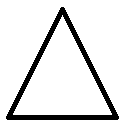
\includegraphics[width=1cm]{tiling_1} is a DET,
  then the equilateral triangle $T'$ built out of four copies of $T$
  as shown in in Figure~\ref{4DET-fig} is also a DET, and the
  subtriangles of $T'$ are exactly the subtriangles of each of the
  copies of $T$.
\end{itemize}

\begin{center}
\begin{figure}\inbook{[h]}
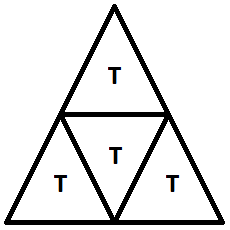
\includegraphics[width=2cm]{tiling_2}
\caption{DET $T'$ from Four Copies of DET $T$}
\label{4DET-fig}
\end{figure}
\end{center}

\bparts

\ppart Define the \emph{length} of a DET to be the number of
subtriangles with an edge on its base.  Prove by induction that the
total number of subtriangles of a DET is the square of its length.

\begin{solution}
The proof will be by strong induction on length.  The induction
hypothesis is that if the length of a DET is $n$, the total number of
subtriangles is $n^2$.

\inductioncase{Base case} ($n = 1$) Here the only subtriangle is the
starting triangle itself, so the total number of subtriangles is $1 = 1^2
= n^2$, proving this case.

\inductioncase{Induction step}: Suppose $T'$ is a DET with base of
length $n>1$.  Then $T'$ must consist of four copies of some DET $T$
as in Figure~\ref{4DET-fig}.  So $n=2k$ where $k$ is the length of
$T$.  Since $k<n$, we have by strong induction hypothesis that $T$ has
$k^2$ subtriangles.  Therefore $T'$ has $4k^2$ subtriangles.  But $4k^2 =
(2k)^2 = n^2$, proving that the number of subtriangles of $T'$ is $n^2$ as
required.

\begin{comment}
Here is a decent false (or just misleading) proof.  Putting it here
for reference Proof by induction\\ Induction hypothesis $P(n)$: a DET
T with $n$ subtriangles with an edge on it's base has $n^2$
subtriangles.\\ \textbf{Base case: $n=1$} There is 1 subtriangle on the base
of T, and $1^2 = 1$ subtriangles total.\\ \textbf{Inductive step:} Assume
by induction that $P(n)$ is true. Then suppose we have a DET with
$n+1$ subtriangles with an edge on its base. Removing the last row of
subtriangles gives us a DET with $n$ subtriangles on its base, and we know by
induction that the number of subtriangles in that portion is $n^2$.
\begin{center}
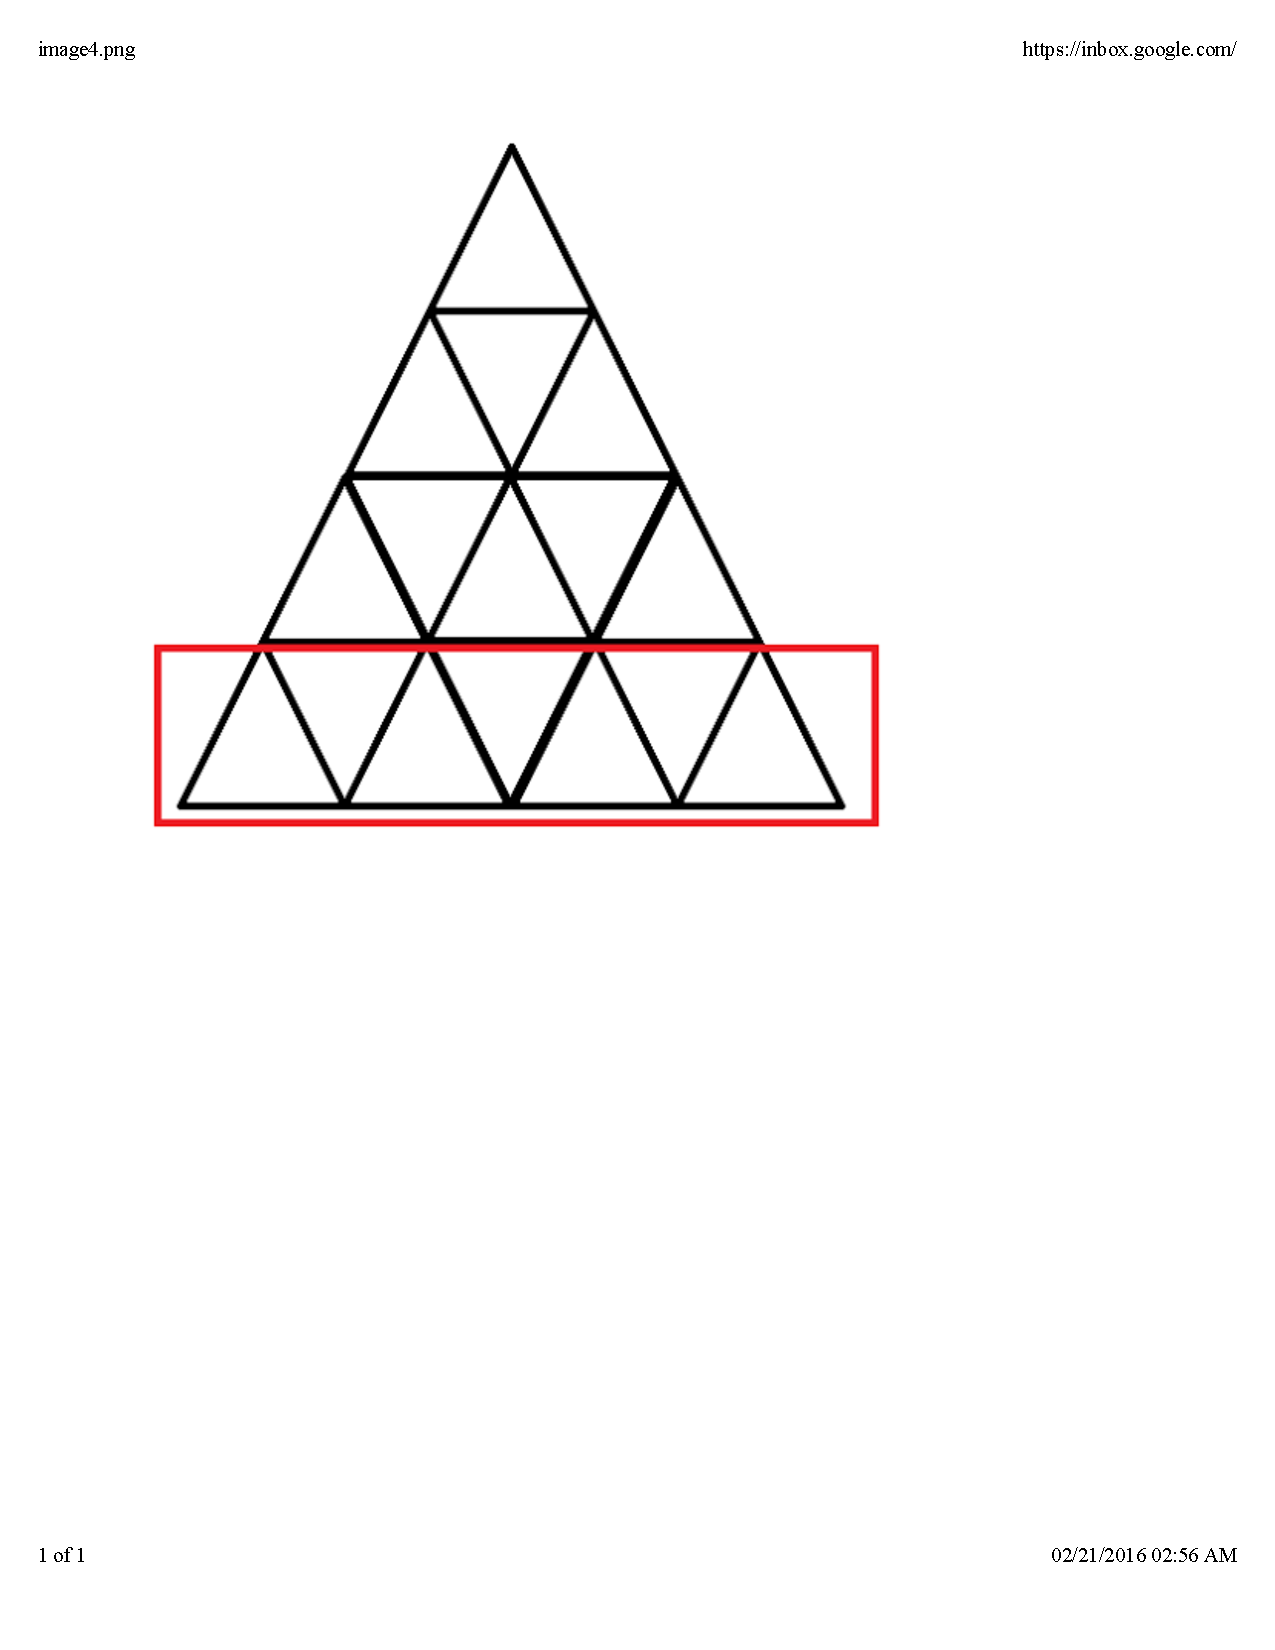
\includegraphics[width=3cm]{tiling_4}
\end{center}
How many subtriangles did we remove? We removed the $n+1$ subtriangles with
edges on the base, and the $n$ subtriangles in between them. So in total
we removed $n+n+1=2n+1$ subtriangles. And so the total number of subtriangles
$= n^2 + 2n + 1 = (n+1)^2$. Thus, $P(n+1)$ is true. Hence, $P(n)$ is
true for all $n$.
\end{comment}

\end{solution}

\ppart Show that a DET with one of its corner subtriangles removed can
be tiled with trapezoids built out of three subtriangles as in
Figure~\ref{3trap-fig}.

\begin{center}
\begin{figure}\inbook{[h]}
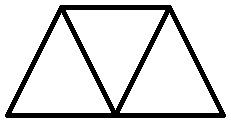
\includegraphics[width=2cm]{tiling_3}
\caption{Trapezoid from Three Triangles}
\label{3trap-fig}
\end{figure}
\end{center}


\begin{solution}
The proof will be by strong induction on length.  The induction  
hypothesis is that if the length of a DET is $n$, and one of its
corner subtriangles is removed, then it can be tiled with trapezoids.

\inductioncase{Base case} ($n = 1$) Here the only subtriangle is the
starting triangle itself, and removing the corner leaves nothing,
which can be tiled with no trapezoids.  This proves the base case.

\inductioncase{Induction step}: Suppose $T'$ is a DET with base of
length $n>1$.  Then $T'$ must consist of four copies of some DET $T$
as in Figure~\ref{4DET-fig}.  So $n=2k$ where $k$ is the length of
$T$.  Since $k<n$, we have by strong induction hypothesis that $T$
with one corner subtriangle can be tiled with trapezoids.

Without loss of generality, we assume that the top corner subtriangle
of $T'$ is removed.  Now remove the right corner of copy 2 of $T$, the
top corner of copy 3, and the left corner of copy 4 as shown in
Figure~\ref{traptile-fig}.  All four copies have one missing corner,
so by strong induction hypothesis they can all be tiled by trapezoids.
The hole left by the middle 3 missing corners can then be tiled with a
single trapezoid, yielding a complete tiling by trapezoids of $T'$
with its top corner removed.

\begin{center}
\begin{figure}\inbook{[h]}
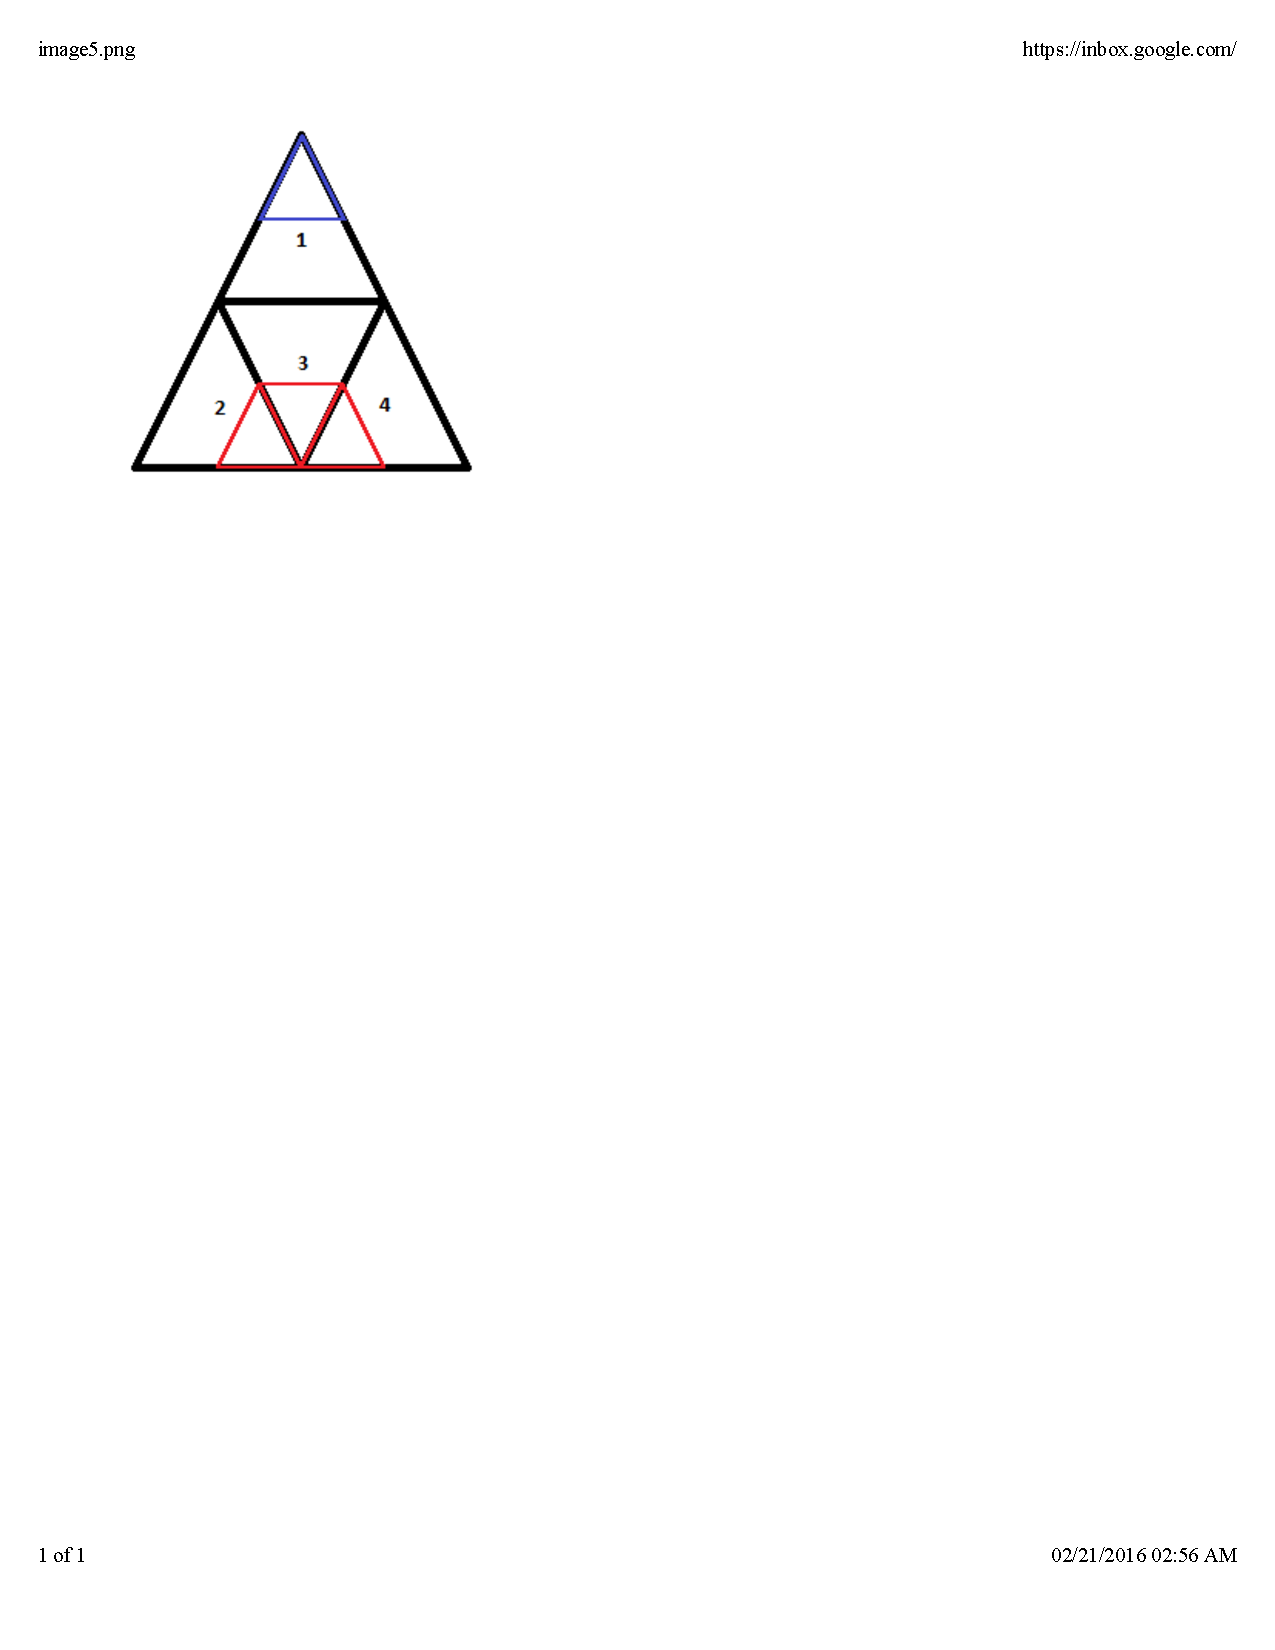
\includegraphics[width=3cm]{tiling_5}
\caption{Tiling $T'$ with trapezoids}
\label{traptile-fig}
\end{figure}
\end{center}

\end{solution}

\eparts

\end{problem}

%%%%%%%%%%%%%%%%%%%%%%%%%%%%%%%%%%%%%%%%%%%%%%%%%%%%%%%%%%%%%%%%%%%%%
% Problem ends here
%%%%%%%%%%%%%%%%%%%%%%%%%%%%%%%%%%%%%%%%%%%%%%%%%%%%%%%%%%%%%%%%%%%%%

\endinput
